\section{生命周期}
在之前的所有权一节,有这么一个函数示例:
\begin{code-block}{rust}
fn first_word(s: &str) -> &str {
    return &s[..];
}

fn copy_ref(s: &str) -> &str {
    // 也可以是&s,为啥?
    return s;
}
\end{code-block}
上述的函数都运行正常。对函数进行改造,改造成下列的样式:
\begin{code-block}{rust}
fn longest(x: &str, y: &str) -> &str {
    if x.len() > y.len() {
        x
    } else {
        y
    }
}
\end{code-block}
即,返回2个字符串当中最长的。如果对这样的代码进行编译,则会出现错误:
\begin{figure}[H]
  \centering
  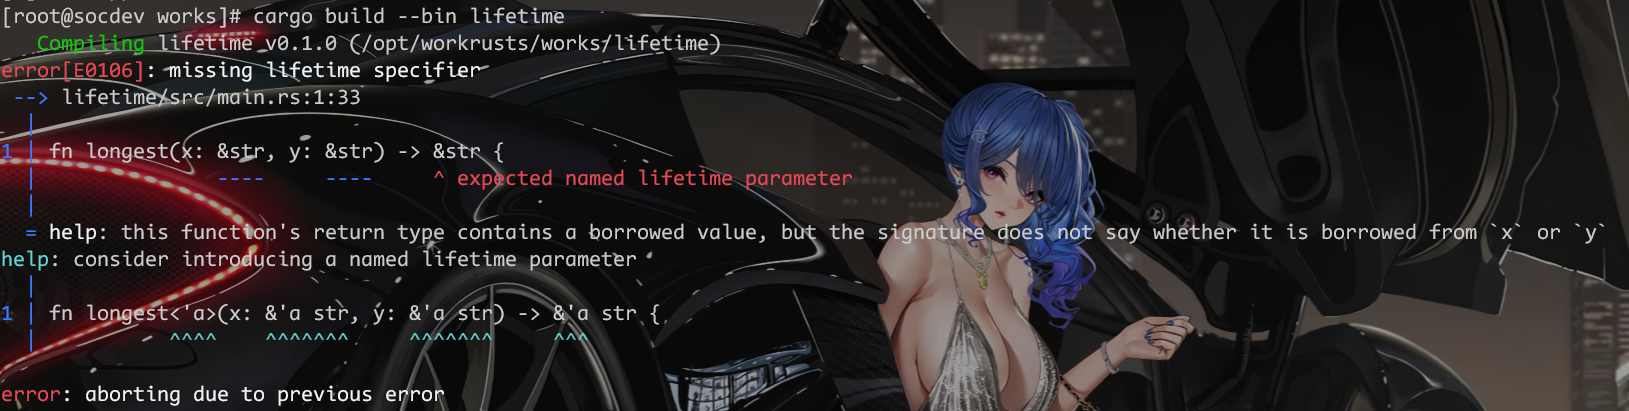
\includegraphics[scale=0.2]{rust_strref_err.png}
  \caption{试图返回多个引用当中的某一个}
  \label{fig:rust_strref_err}
\end{figure}
错误表示,函数应该返回一个有生命周期的命名变量。错误的原因是,Rust编译器无法知道
函数返回的到底是x还是y的引用,无法确定对应的变量的生命周期。
